\chapter{Deeply conserved GWAS SNPs}
\label{chap:zfishSnps}

\section{Introduction}

The NHGRI GWAS catalog (\url{http://www.genome.gov/gwastudies/}) contains
thousands of tag single nucleotide polymorphisms (SNPs) significantly
associated with human diseases and phenotypes collected from hundreds of
independent studies. Up to 90\% of SNPs in this repository lie in
non-genic regions of the genome, and most are thought to highlight
disease-associated modifications to gene regulatory elements~\citep{Hindorff:2009cc}. In addition to
being mostly non-genic, reported SNPs may either be the causal mutation
or may gain their association from linkage with the causal SNP~\citep{Tuupanen:2009dk, Nicolae:2010fk}. Selecting SNPs
under strong sequence conservation across many species has provided a
useful strategy for identifying the causal mutation from multiple
associated loci~\citep{Spieler:2014ky}.
Here we report a computational method to identify human GWAS SNPs
embedded in non-coding DNA elements/regions (CNEs) conserved to
zebrafish, a vertebrate model where the role of these conserved CNE/SNPs
can be studied \emph{in vivo}. In this screen, we require the non-coding
sequences to be conserved syntenically adjacent to the same target
genes. Because sequence conservation is a hallmark of functional
\emph{cis}-regulatory elements~\citep{Hiller:2013hr}, and because these sequences are conserved syntenically, we
hypothesized that our screen would identify causal regulatory mutations
that could be functionally tested in zebrafish.

Our genome-wide screen has identified a first set of 22 such SNPs
covering a wide range of human traits and diseases. We validated the
\emph{cis}-regulatory function of 5/8 human CNEs in the fish and
successfully demonstrated that the risk allele for 3/3 SNPs abolished
enhancer activity and likely contributes to the associated disease. To
further demonstrate the value of our set, we scrutinized CNE1/rs17421627
in more depth. rs17421627 has been associated with retinal vascular
caliber defects in two related GWAS studies searching for novel loci
involved in human vascular diseases and is thought to affect the neighboring
gene, \emph{MEF2C}~\citep{Ikram:2010gv, Sim:2013fm}. Changes in retinal
vascular caliber have been linked with increased cardiovascular risk and
are predictive of global vascular pathology. For example, wider venular
and narrower arteriolar calibers were associated with an increased risk
of coronary heart disease and cardiovascular mortality~\citep{Wang:2007da, McGeechan:2009wc}, while wider
retinal venular caliber also predicted stroke~\citep{McGeechan:2009dr}.

We found that human CNE1 acts as an enhancer and drives expression in
the central nervous system including the retina. We showed that SNP
rs17421627 is a regulatory mutation and that CNE1/rs17421627 regulates
\emph{microRNA-9} expression. miR-9 is a well-known regulator of
neurogenesis~\citep{Coolen:2013dw}.
\emph{In vivo}, miR-9 has been shown to control the proliferation and
differentiation of neural stem cells (NSCs) and its inhibition
transiently increases their proliferation, ultimately resulting in an
increased number of late-differentiating neurons~\citep{Bonev:2011fg, Shibata:2011jm, Coolen:2012gj}. The physiological
role of miR-9 during angiogenesis \emph{in} \emph{vivo} is unknown, but
miR-9 has been associated with cancer cell vascularization \emph{in
vitro}~\citep{Zhang:2012ih, Zhuang:2012jw}. Here, we show that
the deletion of CNE1 ($\Delta$CNE1) in the zebrafish genome and down-regulation
of miR-9 expression leads to retinal vasculature defects similar to risk
allele carriers of rs17421627 in human. Together, our results validate
our \emph{in silico} approach and uncover an unexpected function for
miR-9 in the control of retinal vasculature development. We also
demonstrate that SNP rs17421627 is the causal mutation affecting the
function of CNE1 and responsible for the retinal vascular caliber
phenotype. This illustrates the power of studying non-coding GWAS SNPs
\emph{in vivo} in zebrafish to reveal their biological contributions to
the associated human diseases and phenotypes.

\section{Results}

\subsection{Computational identification of non-coding GWAS SNPs conserved to zebrafish}

\begin{figure}[htbp]
\centering
\begin{tabular}{l}
\epsfig{file=figures/zfishSnpsFigure1.pdf,width=0.99\linewidth,clip=,trim=0 0 0 0} \\
\end{tabular}
\caption[Identification of GWAS SNPs embedded in deeply-conserved non-coding elements]{
{\bf Identification of GWAS SNPs embedded in deeply-conserved non-coding elements.}
{\bf (A)} Methodology used to perform the screen and first list of
regulatory GWAS SNPs conserved between human and zebrafish, and their
conserved syntenic genes. {\bf (B)} The rs17421627 protective allele
and its immediate sequence neighborhood have been conserved across
dozens of species and hundreds of millions of years of evolution,
including in human CNE1 (948 bp; hg19.chr5:87,847,186-87,848,133) and
zebrafish CNE1 (860 bp; danRer7.chr5:49,927,812-49,928,671).
{\bf (C)} The human and zebrafish gene neighborhoods surrounding
CNE1/rs17421627 contain three orthologous and conserved genes:
\emph{TMEM161B}, \emph{MEF2C} and \emph{MIR9-2}. The CNE1/SNP pair is
marked by H3K4me1 and DNase signals in both human fetal brain and
neuronal progenitors.
}
\label{fig:zfishSnpsFig1}
\end{figure}

We began by extracting 14,068 references SNP cluster ID (rsID) entries
from the NHGRI GWAS catalog. We padded each SNP with 100bp on either
side, creating a local sequence context to be used when querying the
zebrafish genome. We then removed all regions overlapping or in close
proximity to any exon to avoid coding and splicing related mutations,
leaving 11,822 GWAS SNP-embedding non-coding elements. For each human
element, we extracted a multiple species alignment block with a varying
number of vertebrate species aligned to the region, constructed a DNA
profile hidden Markov model (HMM), and used nhmmer~\citep{Wheeler:2013gj} to sensitively
query the zebrafish genome. To specifically identify gene regulatory
homologies we then applied a gene synteny filter, requiring that the
human GWAS SNP-embedding region and its top zebrafish alignment are
found near orthologous genes in human and zebrafish (\figref{fig:zfishSnpsFig1} and
Methods in \ref{sec:zfishSnpsMethods}). This resulted in a list of 22 human GWAS SNPs embedded in
non-coding elements conserved in zebrafish next to orthologous genes
(\figref{fig:zfishSnpsFig1}A and \tabref{tab:zfishSnpsTabS1}). The list includes SNPs associated with traits
and diseases ranging from psychiatric to metabolic disorders. To
estimate the false discovery rate (FDR), we used the same set of models
to query the reversed but not complemented zebrafish genome, and this
resulted in zero false positive matches. For 8 of the 22 CNE/SNP pairs,
we identified a single syntenic gene, suggesting the identity of the
gene regulated by the CNE containing the GWAS SNP. Finally, all the CNEs
identified in this screen are strongly conserved during 400 million
years of evolution, suggesting that they are functional
\emph{cis}-regulators (\figref{fig:zfishSnpsFig1}B for an example).

\subsection{Validation of GWAS SNPs embedded in functional enhancers \emph{in vivo}}

\begin{figure}[htbp]
\centering
\begin{tabular}{l}
\epsfig{file=figures/zfishSnpsFigure2.pdf,width=0.7
\linewidth,clip=,trim=0 0 0 0} \\
\end{tabular}
\caption[Functional validation of conserved CNE enhancer
activity and demonstration that the associated SNP can be a regulatory
mutation]{
{\bf Functional validation of conserved CNE enhancer
activity and demonstration that the associated SNP can be a regulatory
mutation.}
{\bf (A)} Schematic of the transgenes carrying the protective and
risk alleles. {\bf (B)} Confocal projections of EGFP immunolabelling
in \emph{Tg(CNE1:egfp)}, \emph{Tg(CNE8:egfp), Tg(CNE10:egfp),
Tg(CNE15:egfp)} and \emph{Tg(CNE18:egfp)}, demonstrating the specific
enhancer activity of these human CNEs in zebrafish. {\bf (C-E)} The
sequences surrounding rs17421627, rs1568679 and rs16932455 are conserved
during evolution. {\bf (C)} Confocal sections of EGFP immunolabelling
in \emph{Tg(CNE1:egfp)} containing the protective allele or
\emph{Tg(CNE1SNP:egfp)} containing the risk allele (rs17421627) in the
adult retina immunolabelled with glutamine synthetase (GS). {\bf (D)}
Confocal projections of EGFP immunolabelling in \emph{Tg(CNE8:egfp)}
containing the protective allele or \emph{Tg(CNE8SNP:egfp)} containing
the risk allele (rs1568679) in the brain of \emph{olig2:dsred2}
transgenic larvae at 72 hpf. {\bf (E)} Confocal projections of EGFP
immunolabelling in \emph{Tg(CNE18:egfp)} containing the protective
allele or \emph{Tg(CNE18SNP:egfp)} containing the risk allele
(rs16932455) in retina immunolabelled with HuC/D at 48 hpf. Dorsal view
of the brain with anterior up. Lateral view of the retina. Scale bars:
100 $\mu$m.
}
\label{fig:zfishSnpsFig2}
\end{figure}

To determine whether the conserved CNE/SNP pairs discovered by our
screen act as \emph{cis}-regulatory elements \emph{in vivo}, we tested
the transcriptional activity of 8 of 22 human CNEs during early
zebrafish development. We fused the human CNE regions to a basal
promoter driving EGFP expression to establish stable zebrafish
transgenic lines (at least 3 independent integrations for each CNE/SNP;
\figref{fig:zfishSnpsFig2}A). We validated enhancer function for 5 of these conserved
non-coding elements (CNE1/rs17421627; CNE8/rs1568679; CNE10/rs12431307;
CNE15/rs11190870; CNE18/rs16932455; \figref{fig:zfishSnpsFig2}B). The lack of activity
observed for three additional CNEs (CNE9, CNE16 and CNE17) could be
attributed to the developmental stage we assayed or, even more
interestingly, their identity as repressor or insulator elements. The
CNEs with validated enhancer function drove restricted EGFP expression
in a variety a cell types (neurons, glial cells, muscles, and
notochord), demonstrating their specific transcriptional activity (\figref{fig:zfishSnpsFig2} and \figref{fig:zfishSnpsFigS1}).

\subsection{The human risk allele abolishes the function of human enhancers \emph{in vivo}}

We next tested the causality of the human risk allele for
CNE1/rs17421627, CNE8/ rs1568679, and CNE18/rs16932455 by introducing the
1 bp change into the 948 bp, 849 bp, and 832bp long human enhancers,
respectively (\figref{fig:zfishSnpsFig2}A). Strikingly, in these 3 enhancers, the risk
allele abolished the transcriptional activity (\figref{fig:zfishSnpsFig2}C-E). In addition,
we performed \emph{in situ} hybridization (ISH) and EGFP immunostaining
to confirm our predictions, and we likely identified the
\emph{cis}-regulated gene for CNE1/\emph{MIR9-2,} CNE8/\emph{MEIS2} and
CNE18/\emph{SOX6} (\figref{fig:zfishSnpsFigS1}), as indicated by the coexpression of EGFP
with the endogenous microRNA or mRNAs. Importantly, a recent report
independently supports our predictions by demonstrating that rs11190870,
associated with scoliosis, is a gain of function mutation regulating
CNE15/\emph{LBX1} activity~\citep{Guo:2016ho}. Overexpression of human \emph{LBX1} or zebrafish \emph{lbx}
genes caused scoliosis~\citep{Guo:2016ho}.
Altogether, these and the above results validate our \emph{in silico}
predictions and demonstrate the approach efficiently identifies causal
CNE/SNP pairs associated with human disease, as well as the genes they
\emph{cis}-regulate.

\subsection{CNE1 enhancer deletion leads to retinal vasculature defects \emph{in vivo}}

\begin{figure}[htbp]
\centering
\begin{tabular}{l}
\epsfig{file=figures/zfishSnpsFigure3.pdf,width=0.7
\linewidth,clip=,trim=0 0 0 0} \\
\end{tabular}
\caption[CNE1 regulates retinal vasculature formation \emph{in
vivo}]{
{\bf CNE1 regulates retinal vasculature formation \emph{in
vivo}.}
{\bf (A)} Schematic of the zebrafish genomic DNA containing CNE1,
which was deleted using the CRISPR/Cas-9 system with a pair of gRNAs
($\Delta$CNE1). The deletion is 770 bp long, including the deeply conserved
sequence of CNE1 (473 bp; danRer7.chr5:49,928,049-49,928,521)
containing the SNP. {\bf (B, C)} CNE1 homozygous mutants display
normal brain and eye morphology {\bf (B)}, but the formation of the hyaloid
vasculature in the retina is affected, as revealed by microangiography
using FITC-dextran injection {\bf (C)}. The retinal vasculature shown in {\bf (C)}
are from larvae shown in {\bf (B)}. {\bf (D)} Confocal projections of
mCherry immunolabelling in \emph{Tg(kdrl:mCherry)} retina at 72 hpf
showing hyaloid vasculature formation in control and ∆CNE1 mutant
larvae. {\bf (E)} Quantification of the hyaloid vasculature network
organization observed in control and ∆CNE1 mutant larvae at 72 hpf. A
minimum of 28 retinas were analyzed for each context. Dorsal view of the
brain with anterior up. Lateral view of the retina. Scale bars: 10 µm.
Error bars represent s.d. *\emph{p}-value \textless{} 0.05,
**\emph{p}-value \textless{} 0.001, ***\emph{p} \textless{} 0.0005, determined by
\emph{t}-test.
}
\label{fig:zfishSnpsFig3}
\end{figure}

Because rs17421627 is a loss of function mutation of CNE1 activity (\figref{fig:zfishSnpsFig2}C and \figref{fig:zfishSnpsFig4}B), we deleted CNE1 in the zebrafish genome to investigate
the function of this conserved enhancer in retinal vasculature
formation. Taking advantage of the CRISPR/Cas-9 system~\citep{Varshney:2015jc}, we deleted 770 bp
of CNE1 (\figref{fig:zfishSnpsFig3}A), including the deeply-conserved region of 473 bp
containing the SNP (\figref{fig:zfishSnpsFig1}B). We used the CNE1 deletion mutant as a
model to study the human CNE1 risk allele phenotype. CNE1 mutants
display normal eye~morphology (\figref{fig:zfishSnpsFig3}B), but micro-angiography of ∆CNE1
larvae revealed a disrupted blood vessel network and vascular defects in
the retina (\figref{fig:zfishSnpsFig3}C), consistent with the human phenotype associated
with the risk allele. We characterized this phenotype using the
\emph{kdrl} (\emph{vegfr2}) reporter line labeling the vasculature~\citep{Chi:2008dw}. We observed a reduction
of \textasciitilde{}40\% in the number of vessels and branching points
in the ∆CNE1 mutant, and the remaining vessels appear to be thicker
(\figref{fig:zfishSnpsFig3}D, E). These results indicate that CNE1 is functionally
associated with blood vessel development in the retina. Our data also
suggest that SNP rs17421627 may be a causal mutation affecting CNE1
activity and responsible for the retinal vascular defects in human.

\begin{figure}[htbp]
\centering
\begin{tabular}{l}
\epsfig{file=figures/zfishSnpsFigure4.pdf,width=0.7
\linewidth,clip=,trim=0 0 0 0} \\
\end{tabular}
\caption[CNE1 enhancer activity is similar to \emph{miR-9}
expression, but not \emph{mef2cb} or \emph{tmem161b}]{
{\bf CNE1 enhancer activity is similar to \emph{miR-9}
expression, but not \emph{mef2cb} or \emph{tmem161b}.}
{\bf (A)} Schematic of the human and zebrafish genomic DNA containing
CNE1 where SNP rs17421627 is located. {\bf (B)} Confocal projections
of EGFP immunolabelling in \emph{Tg(CNE1:egfp)} containing the
protective T allele or \emph{Tg(CNE1SNP:egfp)} containing the risk G
allele (rs17421627) in larvae at 72 hpf. In \emph{Tg(CNE1:egfp)}, EGFP
expression is detected in cell bodies in the inner nuclear layer of the
retina, telencephalon, optic tectum, and hindbrain. The
\emph{Tg(CNE1:egfp)} expression pattern is reminiscent of \emph{miR-9}
expression. EGFP expression in the CNS is abolished in the presence of
the SNP rs17421627 risk allele. {\bf (C)} Whole-mount \emph{in situ}
hybridization against \emph{tmem161b, mef2cb}, and \emph{miR-9} in larvae
at 72 hpf. {\bf (D)} Confocal section of double \emph{in
situ}/immunolabelling showing extensive overlap (arrowheads) in the
expression of endogenous \emph{miR-9} and EGFP protein in
\emph{Tg(CNE1:egfp)} retina at 72 hpf. {\bf (E)} Whole-mount \emph{in
situ} hybridization against miR-9 in zebrafish (2 months old) or mouse
(P2 stage) showing similar expression in the inner nuclear layer of the
retina. Retina (R), Ganglion cells layer (GCL), Inner nuclear layer
(INL), Telencephalon (T), Optic Tectum (OT), Hindbrain (H). Dorsal view
of the brain with anterior up. Lateral view of the retina. Scale bars:
100 $\mu$m.
}
\label{fig:zfishSnpsFig4}
\end{figure}

\subsection{CNE1 enhancer regulates \emph{MIR-9-2/miR9-5} expression}

CNE1/rs17421627 occupies open chromatin in human fetal brain cells (\figref{fig:zfishSnpsFig1}C), suggesting that it is active and regulates a syntenically-conserved
neighboring gene in the central nervous system. Consistent with this
observation, the human CNE1 (948 bp) used to establish \emph{CNE1:egfp}
transgenic zebrafish drove EGFP expression in the brain and retina (\figref{fig:zfishSnpsFig4}B and \figref{fig:zfishSnpsFigS1}B, C). The SNP is located \textasciitilde{}283 kilobase pairs (kb) and
\textasciitilde{}352 kb away from the closest neighboring coding genes in
the human genome, \emph{TMEM161B} and \emph{MEF2C} respectively (\figref{fig:zfishSnpsFig4}A). In both GWAS studies that replicated rs17421627~\citep{Ikram:2010gv, Sim:2013fm}, the authors
hypothesized \emph{MEF2C} to be the affected target gene because of its
role in cardiovascular development~\citep{Lin:1997vi}. However, the \emph{CNE1:egfp} expression profile matched
neither the \emph{tmem161b} nor \emph{mef2cb} mRNA expression patterns
revealed by whole mount \emph{in situ} hybridization at the same stage
(\figref{fig:zfishSnpsFig4}C). Our own \emph{in silico} predictions, which included both coding and non-coding
gene synteny checks, suggested a third candidate target gene of CNE1,
the \emph{MIR-9-2} microRNA (\figref{fig:zfishSnpsFig1}A). This microRNA was originally not
well annotated, which may explain its absence in the original GWAS.
\emph{MIR-9-2} is located \textasciitilde{}147 kb away from CNE1 and is
in fact closer to CNE1 than both \emph{MEF2C} and \emph{TMEM161B}.
\emph{miR-9-5}, the zebrafish ortholog of the human \emph{MIR-9-2}, is
also the closest conserved adjacent gene to CNE1 in the zebrafish genome
(\figref{fig:zfishSnpsFig1}C and \figref{fig:zfishSnpsFig4}A). We next performed ISH against \emph{miR-9} in
zebrafish larvae and adults, and we found that \emph{miR-9} is expressed
in the brain and retina in a pattern very similar to \emph{CNE1:egfp}
(\figref{fig:zfishSnpsFig4}B-D and \figref{fig:zfishSnpsFigS1}A-C). Importantly, \emph{miR-9} colocalized with
EGFP in the \emph{CNE1:egfp+} cells in the brain and retina (\figref{fig:zfishSnpsFig4}D and
\figref{fig:zfishSnpsFigS1}B, C), supporting that \emph{MIR-9-2}/\emph{miR-9-5} could be a
\emph{cis}-regulatory target of CNE1. Furthermore, consistent with the
human retina phenotype, \emph{MIR-9} expression has been reported in human
retina extracts~\citep{Karali:2016db}.
Here we found that \emph{miR-9} genes expression is conserved in the
inner nuclear layer of both the zebrafish and mouse retina (\figref{fig:zfishSnpsFig4}E).

\begin{figure}[htbp]
\centering
\begin{tabular}{l}
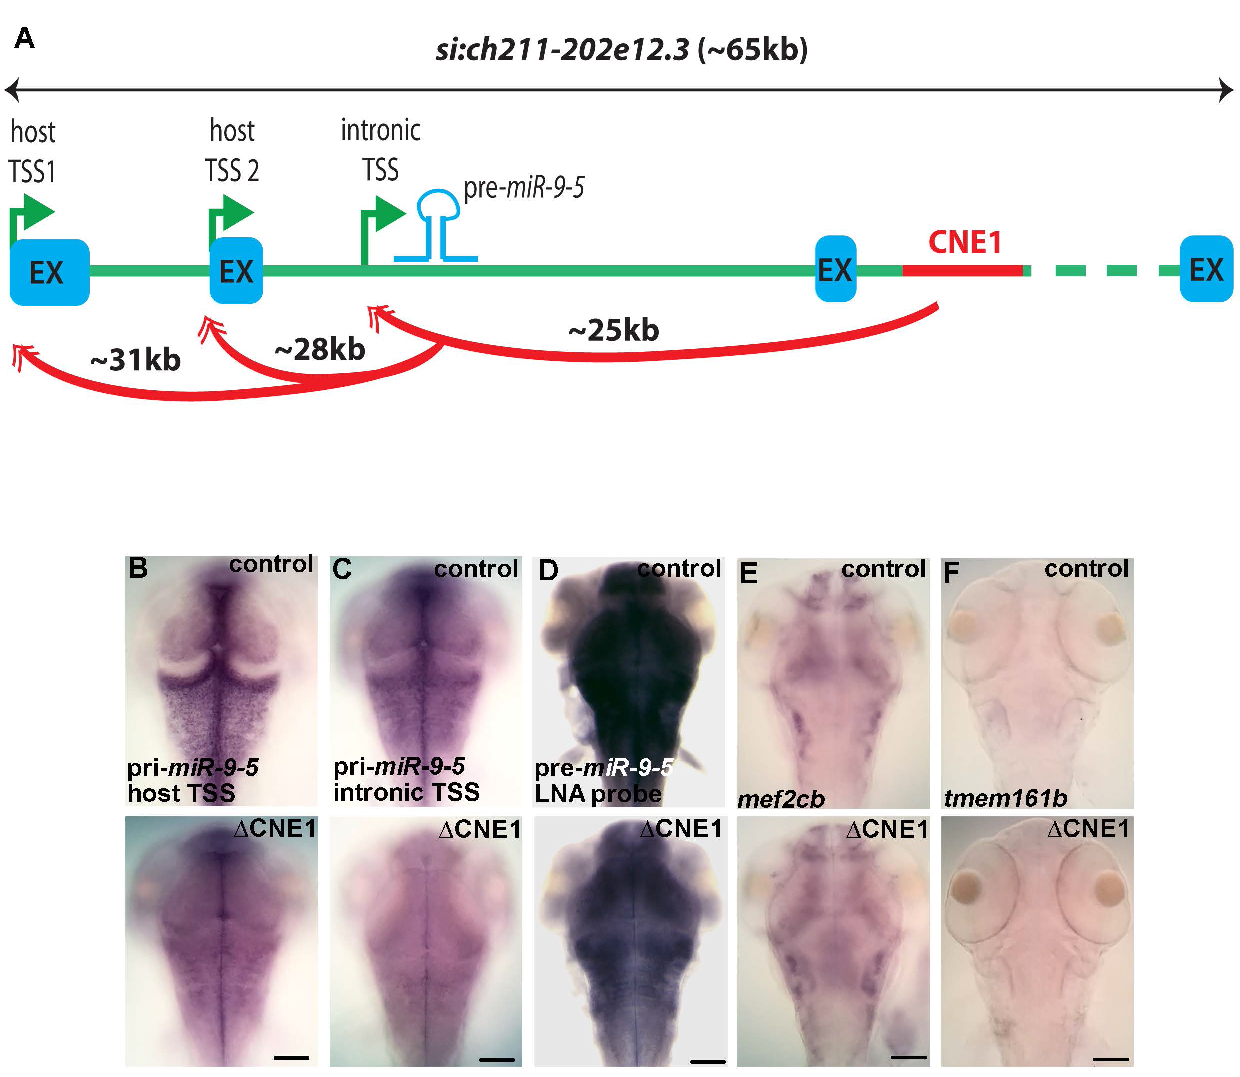
\epsfig{file=figures/zfishSnpsFigure5.pdf,width=0.7
\linewidth,clip=,trim=0 0 0 0} \\
\end{tabular}
\caption[CNE1 regulates \emph{MIR-9-2}/\emph{miR-9-5}
expression]{
{\bf CNE1 regulates \emph{MIR-9-2}/\emph{miR-9-5}
expression.}
{\bf (A)} Schematic of the zebrafish genomic region containing
pre-\emph{miR-9-5} and CNE1\emph{.} pre\emph{-miR-9-5} and CNE1 are
intronic in \emph{si:ch211-202e12.3}, a long non-coding RNA. Three
transcription start sites (TSS, green arrows), host and intronic, are used
for pri-\emph{miR-9-5} transcription~\citep{Nepal:2016hm}. {\bf (B-F)}
Whole-mount \emph{in situ} hybridization against host and intronic
pri\emph{-miR-9-5s,} pre-\emph{miR-9-5}, \emph{tmem161b}, or \emph{mef2c}
in control and $\Delta$CNE1 larvae at 72 hpf. The expression of pri- and
pre-\emph{miR-9-5}, but not \emph{tmem161b} or \emph{mef2c}, is reduced
in the brain of ∆CNE1 mutants. Dorsal view of the brain with anterior
up. Scale bars: 100 $\mu$m.
}
\label{fig:zfishSnpsFig5}
\end{figure}

We next tested whether CNE1 is an actual \emph{cis}-regulator of
\emph{MIR-9-2}/\emph{miR-9-5} by examining \emph{miR-9-5} expression in
∆CNE1 mutant larvae. In both human and zebrafish,
\emph{MIR-9-2}/\emph{miR-9-5} is part of long non coding pri-miRNAs~\citep{Rodriguez:2004kc, Pauli:2012ip}, \emph{LINC00461} and
\emph{si:ch211-202e12.3} respectively (\figref{fig:zfishSnpsFig1}C and \figref{fig:zfishSnpsFig5}A). In both
species CNE1 is intronic to these pri-miRNA genes (\figref{fig:zfishSnpsFig1}C  and \figref{fig:zfishSnpsFig5}A),
suggesting that CNE1 could act as an enhancer of these \emph{LINCs}. In
zebrafish though, it was recently shown that \emph{miR-9-5} comes from
the processing of this long host pri-miRNA in addition to an alternative
intronic promoter located 1.1 kb upstream of the pre-\emph{miR-9-5}
sequence~\citep{Nepal:2016hm}. Using
specific riboprobes, Nepal and colleagues showed that transcripts from
the host and intronic promoters have the same onset of expression (14
somite stage) and the same spatial distribution in the CNS, suggesting
transcriptional co-regulation. Using similar riboprobes, we found a
reduction in the expression of both \emph{miR-9-5} precursors in ∆CNE1
mutant larvae (\figref{fig:zfishSnpsFig5}B, C), suggesting that CNE1 acts as an enhancer
shared by both the host and intronic promoters. We then confirmed that
the down-regulation of \emph{miR-9-5} pri-precursors in ∆CNE1 led to a
specific reduction of pre-\emph{miR-9-5} by using a LNA probe that
specifically distinguished pre-\emph{miR-9-5} from the other mature
miR-9 sequences (\figref{fig:zfishSnpsFig5}D). Finally, we showed that at this stage CNE1
likely acts as a specific enhancer of \emph{MIR-9-2}/\emph{miR-9-5,} as
\emph{tmem161b} and \emph{mef2cb} expression patterns were unaffected in
∆CNE1 mutants (\figref{fig:zfishSnpsFig5}E, F). Thus, these data suggest that the causal
impact of SNP rs17421627 mutation on the human retinal vasculature is
likely due to the downregulation of \emph{MIR-9-2}.

\subsection{miR-9 depletion leads to retinal vasculature formation
defects}

Because miR-9 is a well-known regulator of neurogenesis~\citep{Coolen:2013dw}, the putative
involvement in vasculature formation came as a surprise, as we did not
detect any expression in endothelial cells (ECs) or blood vessels (\figref{fig:zfishSnpsFigS2} and Prof. Bally-Cuif, personal communication). Consistent with these
observations, \emph{LINC00461}, the human \emph{MIR-9-2} precursor~\citep{Rodriguez:2004kc}, is not expressed
in ECs in the human brain
(\url{http://www.brainrnaseq.org})~\citep{Zhang:2016bm}. Similarly, we only
detected miR-9 in neural cells in zebrafish (\figref{fig:zfishSnpsFig2}C and \figref{fig:zfishSnpsFig4}D).
However, previous \emph{in vitro} studies associated \emph{miR-9}
expression with tumor angiogenesis~\citep{Zhang:2012ih, Zhuang:2012jw},
suggesting that miR-9 activity could have a role during physiological
retinal angiogenesis, potentially through the neurovascular link~\citep{Quaegebeur:2011bd}.

\begin{figure}[htbp]
\centering
\begin{tabular}{l}
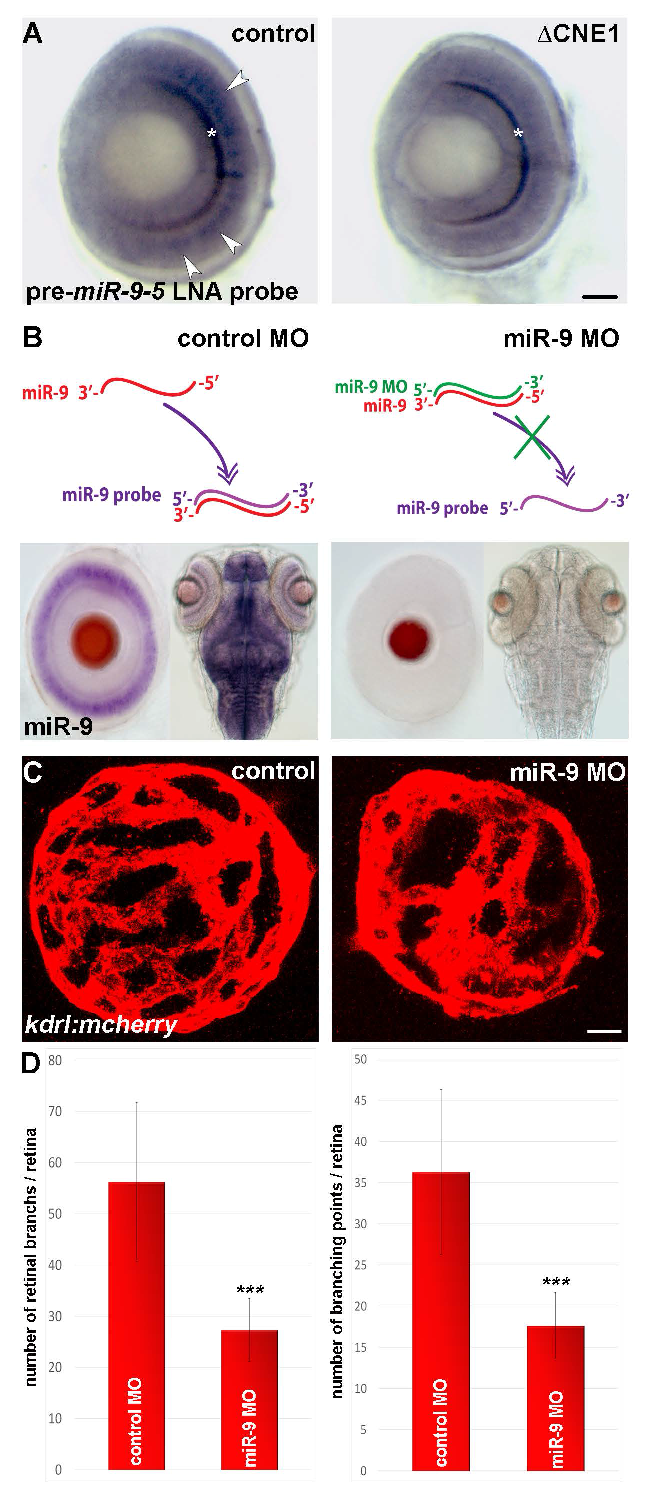
\epsfig{file=figures/zfishSnpsFigure6.pdf,width=0.35
\linewidth,clip=,trim=0 0 0 0} \\
\end{tabular}
\caption[miR-9 controls retinal vasculature development]{
{\bf miR-9 controls retinal vasculature development.}
{\bf (A)} Whole-mount \emph{in situ} hybridization against
pre-\emph{miR-9-5} in control and ∆CNE1 mutant retina at 72 hpf. In 88\%
of the mutant retinas (n=43), \emph{miR-9-5} expression is reduced or
absent, compared to the control larvae (n=34). Arrowheads show
\emph{miR-9-5} expression in the inner nuclear layer of the retina.
Asterisk shows background staining with the pre-\emph{miR-9-5} LNA
probe. This unspecific staining site is not observed with the mature
miR-9 LNA probe (see \figref{fig:zfishSnpsFig4}C and \figref{fig:zfishSnpsFig6}B). {\bf (B)} Schematic
representation of the miR-9 MO binding to microRNA-9. With the control
MO, miR-9 is freely available revealing the miR-9 expression pattern
with the specific miR-9 LNA probe. In presence of the miR-9 MO, miR-9 is
bound by the MO inhibiting the binding of the LNA probe. miR-9 morphant
larvae show no obvious defects in the brain and eye morphogenesis
compared to the control MO. {\bf (C)} Confocal projections of mCherry
immunolabelling in \emph{Tg(kdrl:mCherry)} retina at 72 hpf showing
hyaloid vasculature formation in control MO and miR-9 MO injected
larvae. {\bf (D)} Quantification of the hyaloid vasculature network
organization observed in the control MO or the miR-9 MO at 72 hpf. A
minimum of 24 retinas was analyzed for each context. Dorsal view of the
brain with anterior up. Lateral view of the retina. Scale bars: 100 $\mu$m
(A) or 10 $\mu$m (C). Error bars represent s.d. *\emph{p}-value \textless{} 0.05,
**\emph{p}-value \textless{} 0.001, ***\emph{p}-value \textless{} 0.0005, determined by \emph{t}-test.
}
\label{fig:zfishSnpsFig6}
\end{figure}

To investigate whether \emph{miR-9} down-regulation is involved to a
retinal vascular phenotype, we analyzed the expression of the
pre-\emph{miR-9-5} in the retina of ∆CNE1 mutant larvae. \emph{miR-9-5}
expression is absent in mutant retinas (\figref{fig:zfishSnpsFig6}A), indicating that a
down-regulation of \emph{miR-9} expression may be responsible for the
retinal blood vessel defects observed in ∆CNE1 mutants. To further
support the causal function of~miR-9 in retinal angiogenesis \emph{in
vivo}, we used the previously described miR-9 morpholino~\citep{Leucht:2008ha, Coolen:2013dw} to knockdown its
expression in \emph{kdrl:mCherry} revealing the vasculature~\citep{Chi:2008dw}. miR-9~morphants display
normal brain and eye~morphology (\figref{fig:zfishSnpsFig6}B), but the hyaloid vasculature
in the retina was strongly reduced and the remaining vessels were
thicker (\figref{fig:zfishSnpsFig6}C). We characterized this reduction in blood vessel
branching complexity and observed a decrease of \textasciitilde{}50\% in
the number of retinal vessels and branching points (\figref{fig:zfishSnpsFig6}D), indicating
that the vascular network organization is affected in the retina. These
results demonstrate that miR-9 expression is required for the normal
development of the retinal vasculature. Altogether our data show that
the rs17421627 risk allele abolishes CNE1 \emph{cis}-enhancer regulation
of \emph{MIR9-2}, and \emph{MIR-9} downregulation is very likely
responsible for the retinal blood vessel defects in human.

\section{Discussion}

This work discovered 22 human phenotype-associated regulatory SNPs that
are embedded within sequences conserved to zebrafish, a vertebrate
system where we model one such SNP's functional impact and the biology
of the associated human phenotype \emph{in vivo}. With the growth of the
NHGRI GWAS Catalog driven by larger cohort studies implicating more SNPs
that reach genome-wide significance~\citep{SchizophreniaWorkingGroupofthePsychiatricGenomicsConsortium:2014eb}, we expect the number of GWAS SNPs conserved
to zebrafish and the utility of our approach to grow. Moreover, similar
screens can be performed in other valuable model organisms like \emph{Xenopus} (separated hundreds of millions of years from zebrafish)
to provide dozens of additional high quality \emph{cis}-targets for
studying \emph{in vivo}.

Determining the biological implications of GWAS SNPs remains a
challenge. The overwhelming majority of the GWAS SNPs identified (90\%
of \textasciitilde{}14k SNPs) occupy non-genic portions of the genome
that do not result in an obvious disruption, such as causing a
non-synonymous amino acid change within a protein coding gene, making
them challenging to interpret. Furthermore, GWAS studies report tag SNPs
that may be merely co-segregating markers with the casual mutation~\citep{Tuupanen:2009dk, Nicolae:2010fk}. Our screen takes on
these challenges. The evolutionary distance between human and zebrafish
can reveal non-coding SNPs of likely importance for gene
\emph{cis}-regulation~\citep{Hiller:2013hr}. A hallmark of \emph{cis}-regulatory sequence conservation is
that it persists alongside the gene or genes it regulates, even in
species as diverged as human and zebrafish, a property which we
exploited in our computational screen. This allowed us to include very
sensitive alignments while maintaining an estimated zero
false-positives. By identifying aligning non-coding regions adjacent to
orthologous genes, we also predict the putative target genes whose
expression may be modulated by the regulatory SNPs. In some cases, our
predicted target genes (but not our CNEs) have already been implicated
in the GWAS phenotype itself. For example, the predicted target gene of
CNE12/rs13095226, associated with macular degeneration, is
\emph{COL8A1}, in which mutations are known to cause cornea
abnormalities~\citep{Hopfer:2005gy}.
Likewise, we link severe myopia CNE13/rs13382811 to \emph{ZEB2}, in
which mutations are known to deform lens morphology~\citep{Manthey:2014fy}.

While our approach cannot comprehensively address the problem of
interpreting all non-genic GWAS SNPs, it provides a tractable approach
for functionally studying a fair number of them in zebrafish. The first
22 GWAS SNPs revealed by our genomic screen are associated with a wide
variety of human phenotypes and diseases, which range from drug
responses to cancer to mental illnesses. Studying these polymorphic
sites in zebrafish provides an attractive first step in deciphering the
biological mechanisms underpinning the human traits. In addition to
CNE1/rs17421627, we validated the specific transcriptional activity and
the regulatory activity of the SNPs found in other conserved CNEs.
CNE18/rs16932455 drives EGFP expression in retinal ganglion cells of the
retina and in muscles of the trunk, where \emph{sox6} mRNA is also
expressed and is important during development~\citep{Jackson:2015gu}. CNE10 activity is
observed in the notochord, and \emph{spry2}, the predicted
\emph{cis}-regulated gene, is known to be involved in the formation of
this structure~\citep{Sivak:2005by}.
Furthermore, EGFP driven by CNE8/rs1568679, associated to antipsychotic
response, co-localizes with \emph{meis2} mRNA in the zebrafish brain and
a recent study demonstrated that CNE15/rs11190870 regulates \emph{LBX1}
and is responsible for the associated scoliosis disease~\citep{Guo:2016ho}. Further investigations
are needed to shed light on the role of these CNE/SNP pairs in the
associated human disorders. This study also demonstrated the efficiency
of a targeted deletion of the conserved CNE1 in the zebrafish genome
using the CRISPR/Cas-9 system. This genome editing technique may also be
promising for the CNEs without enhancer activity (CNE9, CNE16 and
CNE17), as it may reveal endogenous repressor/insulator functions.
Together, these data demonstrated the efficiency of the zebrafish as a
model system to validate the activity of human CNEs and the regulatory
role of SNPs, as well as study the biology of the associated human
diseases. Our study of the \emph{miR-9} CNE/SNP pair in zebrafish
illustrates the necessity of working with an animal model system, in
addition to cell culture, to reveal the impact on gene regulation at the
whole organism level.

Our experiments also revealed numerous insights on the functional impact
and biology of the \emph{miR-9-}regulating CNE/SNP. First, a human CNE
of only several hundred bases can drive a very precise expression
pattern in space and time during zebrafish development, demonstrating
the specificity of the enhancer. Second, the mutagenic potential of a
risk allele can be directly tested in fish allowing us to discriminate
between a co-segregating variant and the causal mutation. Third, by
comparing the enhancer reporter expression with the mRNA distribution of
the neighboring genes and by deleting the CNE in the zebrafish genome,
we identified the actual \emph{cis}-regulated gene. Finally, our
findings revealed that the microvasculature defect studied in the GWAS
is the result of \emph{MIR-9-2} expression downregulation in neural
cells and uncover a function for miR-9 during angiogenesis \emph{in
vivo}. This study illustrates how the combination of human and model
organism genetics can reveal unexpected biological processes regulated
by causal SNP mutations.

\section{Methods}
\label{sec:zfishSnpsMethods}

\subsection{Identification of zebrafish conserved non-coding GWAS
SNPs}

The NHGRI GWAS catalog (\url{http://www.genome.gov/gwastudies/}) was most
recently downloaded on October 7, 2014. rsIDs were extracted from the
catalog and mapped to genomic loci in the GRCh37 human reference (hg19)
using the dbSNP 137 database~\citep{Sherry:2001tj} table from the UCSC Genome Browser~\citep{Karolchik:2014eu}. Only uniquely
mapping rsIDs were retained. Each SNP was padded with 100 bp on each
side, creating a local sequence context to be used when querying the
zebrafish genome. Those elements overlapping any (coding or non-coding)
Ensembl exon (Ensembl release 75)~\citep{Flicek:2014cy}, padded by 50 bp, were excluded to avoid all coding and
splicing related events (while non-coding intronic sequences were not
removed).

For each element, the corresponding alignment blocks from a varying
number of species were extracted from the UCSC 46-way multiple alignment~\citep{Karolchik:2014eu}. Sequences that
had been soft-masked in the UCSC alignment were hard-masked to prevent
alignments between repetitive sequences. A profile HMM was constructed
from the alignment corresponding to each element using the hmmbuild
utility from the HMMER package (version 3.1b1)~\citep{Wheeler:2013gj}. This model was
used to query the zebrafish Zv9 assembly (danRer7) using nhmmer (version
3.1b1) with default parameters. All alignments were retained. The human
and zebrafish matches were then realigned using LASTZ (version 1.02.00;
-\/-seed=match4 -\/-hspthresh=500 -\/-gappedthresh=500; HoxD55 scoring
matrix; \url{http://www.bx.psu.edu/~rsharris/lastz/}). Only pairs
scoring above 2000 were retained.

GWAS SNPs embedded specifically in gene regulatory regions conserved to
zebrafish are expected to lie next to the orthologous gene(s) in both
human and zebrafish. This property is known as synteny. Ensembl gene
transcripts and ortholog mappings (Ensembl release 75)~\citep{Flicek:2014cy} were used to
identify syntenic alignments. The top-scoring zebrafish alignment for
each human query was labeled as syntenic if there exists an Ensembl gene
transcript within 500kb of the hg19 SNP, as well as an Ensembl gene
transcript corresponding to a human gene ortholog within 500kb of the
zebrafish alignment.

\subsection{CRISPR/Cas-9 deletion of CNE1 in the zebrafish genome}

To delete CNE1, we took advantage of the previously described genome
editing protocol~\citep{Varshney:2015jc}.
We used two gRNA targeting the CNE1 locus (5'-CCCGGCGTCCCCCT-TCCT-3' and
5'-AGGAAGGGGGACGCCGGG-3'). Co-injection of these gRNAs with the
\emph{Cas9} mRNA resulted in a deletion of 770 bp removing CNE1 most
conserved core including SNP position. F0 carriers for the deletion in
the germ line were first screened by PCR on F1 embryo mix. Identified
carriers were then out-crossed to obtain F1 heterozygous mutants. F2
mutants homozygous for the deletion were also confirmed by PCR and
sequencing.

\subsection{Fish lines and developmental conditions}

Embryos were raised and staged according to standard protocols~\citep{Kimmel:1995kn} and in accordance
with Stanford University animal care guidelines. The following
transgenic lines were used: \emph{Tg(kdrl:ras-mCherry})~\citep{Kimmel:1995kn}, \emph{Tg(kdrl:egfp})~\citep{Choi:2007dn}, and
\emph{Tg(olig2:dsred2})~\citep{Kucenas:2008ec}. Embryos were fixed overnight at 4$^\circ$C in 4\%
paraformaldehyde/1xPBS, after which they were dehydrated through an
ethanol series and stored at −20$^\circ$C until use.

\subsection{Plasmid construction and transgenic line establishment}

For the generation of \emph{Tg(CNEx:egfp)} and \emph{Tg(CNExSNP:egfp),}
transgenic lines were made by PCR amplification of human genomic DNA.
PCR products were directionally cloned into the XhoI and BglII sites of
the pTol2-E1b:EGFP vector. Plasmids were injected into one-cell stage
embryos with the Tol2 mRNA transposase~\citep{Kwan:2007kh}. For each stable line,
at least 3 independent integrations were used to validate the specific
transcriptional activity or the absence of expression with the risk
allele. For example, for the \emph{Tg(CNE1:egfp),} 4 independent
integrations with an identical EGFP expression pattern were identified.
For the \emph{Tg(CNE1SNP:egfp)}, \emph{Tg(CNE8SNP:egfp)} and
\emph{Tg(CNE18SNP:egfp),} 9, 5 and 4 independent integrations with no
detectable EGFP expression were isolated and analyzed respectively.

\subsection{\emph{In situ} hybridization and immunostaining}

\emph{In situ} hybridizations were performed as previously described~\citep{Oxtoby:1993um}. \emph{meis2a}
and \emph{sox6} ORFs were cloned in a pCS2+ vector using zebrafish cDNA
and antisense DIG labelled probes were transcribed using the linearized
pCS2+ plasmid containing the ORF. For \emph{miR-9} ISH, the previously
described miRCURY detection probe (LNA) hsa--miR-9 (Exiqon) was used~\citep{Leucht:2008ha}. Probes for
\emph{pri-miR-9-5s} were amplified by PCR on genomic DNA to target the
previously described regions in the \emph{miR-9-5} pri-precursors~\citep{Nepal:2016hm}. For
pre-\emph{miR-9-5} ISH, a miRCURY LNA probe (dre-mir-9-5;
TATGAAGTGCAAAATACTC) was specifically designed by Exiqon. \emph{In
situs} were revealed using either BCIP and NBT (Roche) or Fast Red
(Roche) as substrates.

Immunohistochemical stainings were performed as previously described~\citep{Masai:1997eu}, using either
anti-GFP (1/1000, Torrey Pines Biolabs), anti-HuC/D (1/500, Molecular
Probes), anti-glutamine synthetase (1/500, Millipore) or anti-DsRed
(1/500, Clontech) as primary antibodies and Alexa 488 or Alexa
555-conjugated goat anti-rabbit IgG or goat anti-mouse IgG (1/1000) as
secondary antibodies (Molecular Probes). FITC-dextran 2000 kDa (Sigma)
was used to visualize the vasculature after injection in the cardinal
vein.

\subsection{Antisense morpholino injection}

For morpholino knockdowns, we used the previously described miR-9 MO
(TCATACAGCTAGATAACCAAAGA) and the control MO (CACCAAACCATATAGAAGTGATA)
(1mM)~\citep{Leucht:2008ha, Coolen:2012gj}. Embryos were
injected at the one-cell stage with 1-2 nl of the MO.

\subsection{Image acquisition}

Confocal acquisitions were carried out using a Leica SP5 confocal
microscope (Stanford cell science imaging facility). Images were
manipulated using Photoshop (Adobe) software. For quantification,
confocal stacks were analyzed using ImageJ software.
